\subsection{Forward Time-Of-Flight (FTOF)}

\subsection{Geometry}

The FTOF geometry is implemented through the COATJAVA geometry service.
The service provides the Geant4 definitions that are read by the GEMC perl API to build the geometry database.

All scintillators are Geant4 volumes. The paddles are assigned the scintillator material and associated with the FTOF hit process routine.
Each scintillator is a G4Box embedded in a G4Trapezoid mother volume made of air, see \F{ftofGeometry}. 

\begin{figure}
	\centering
	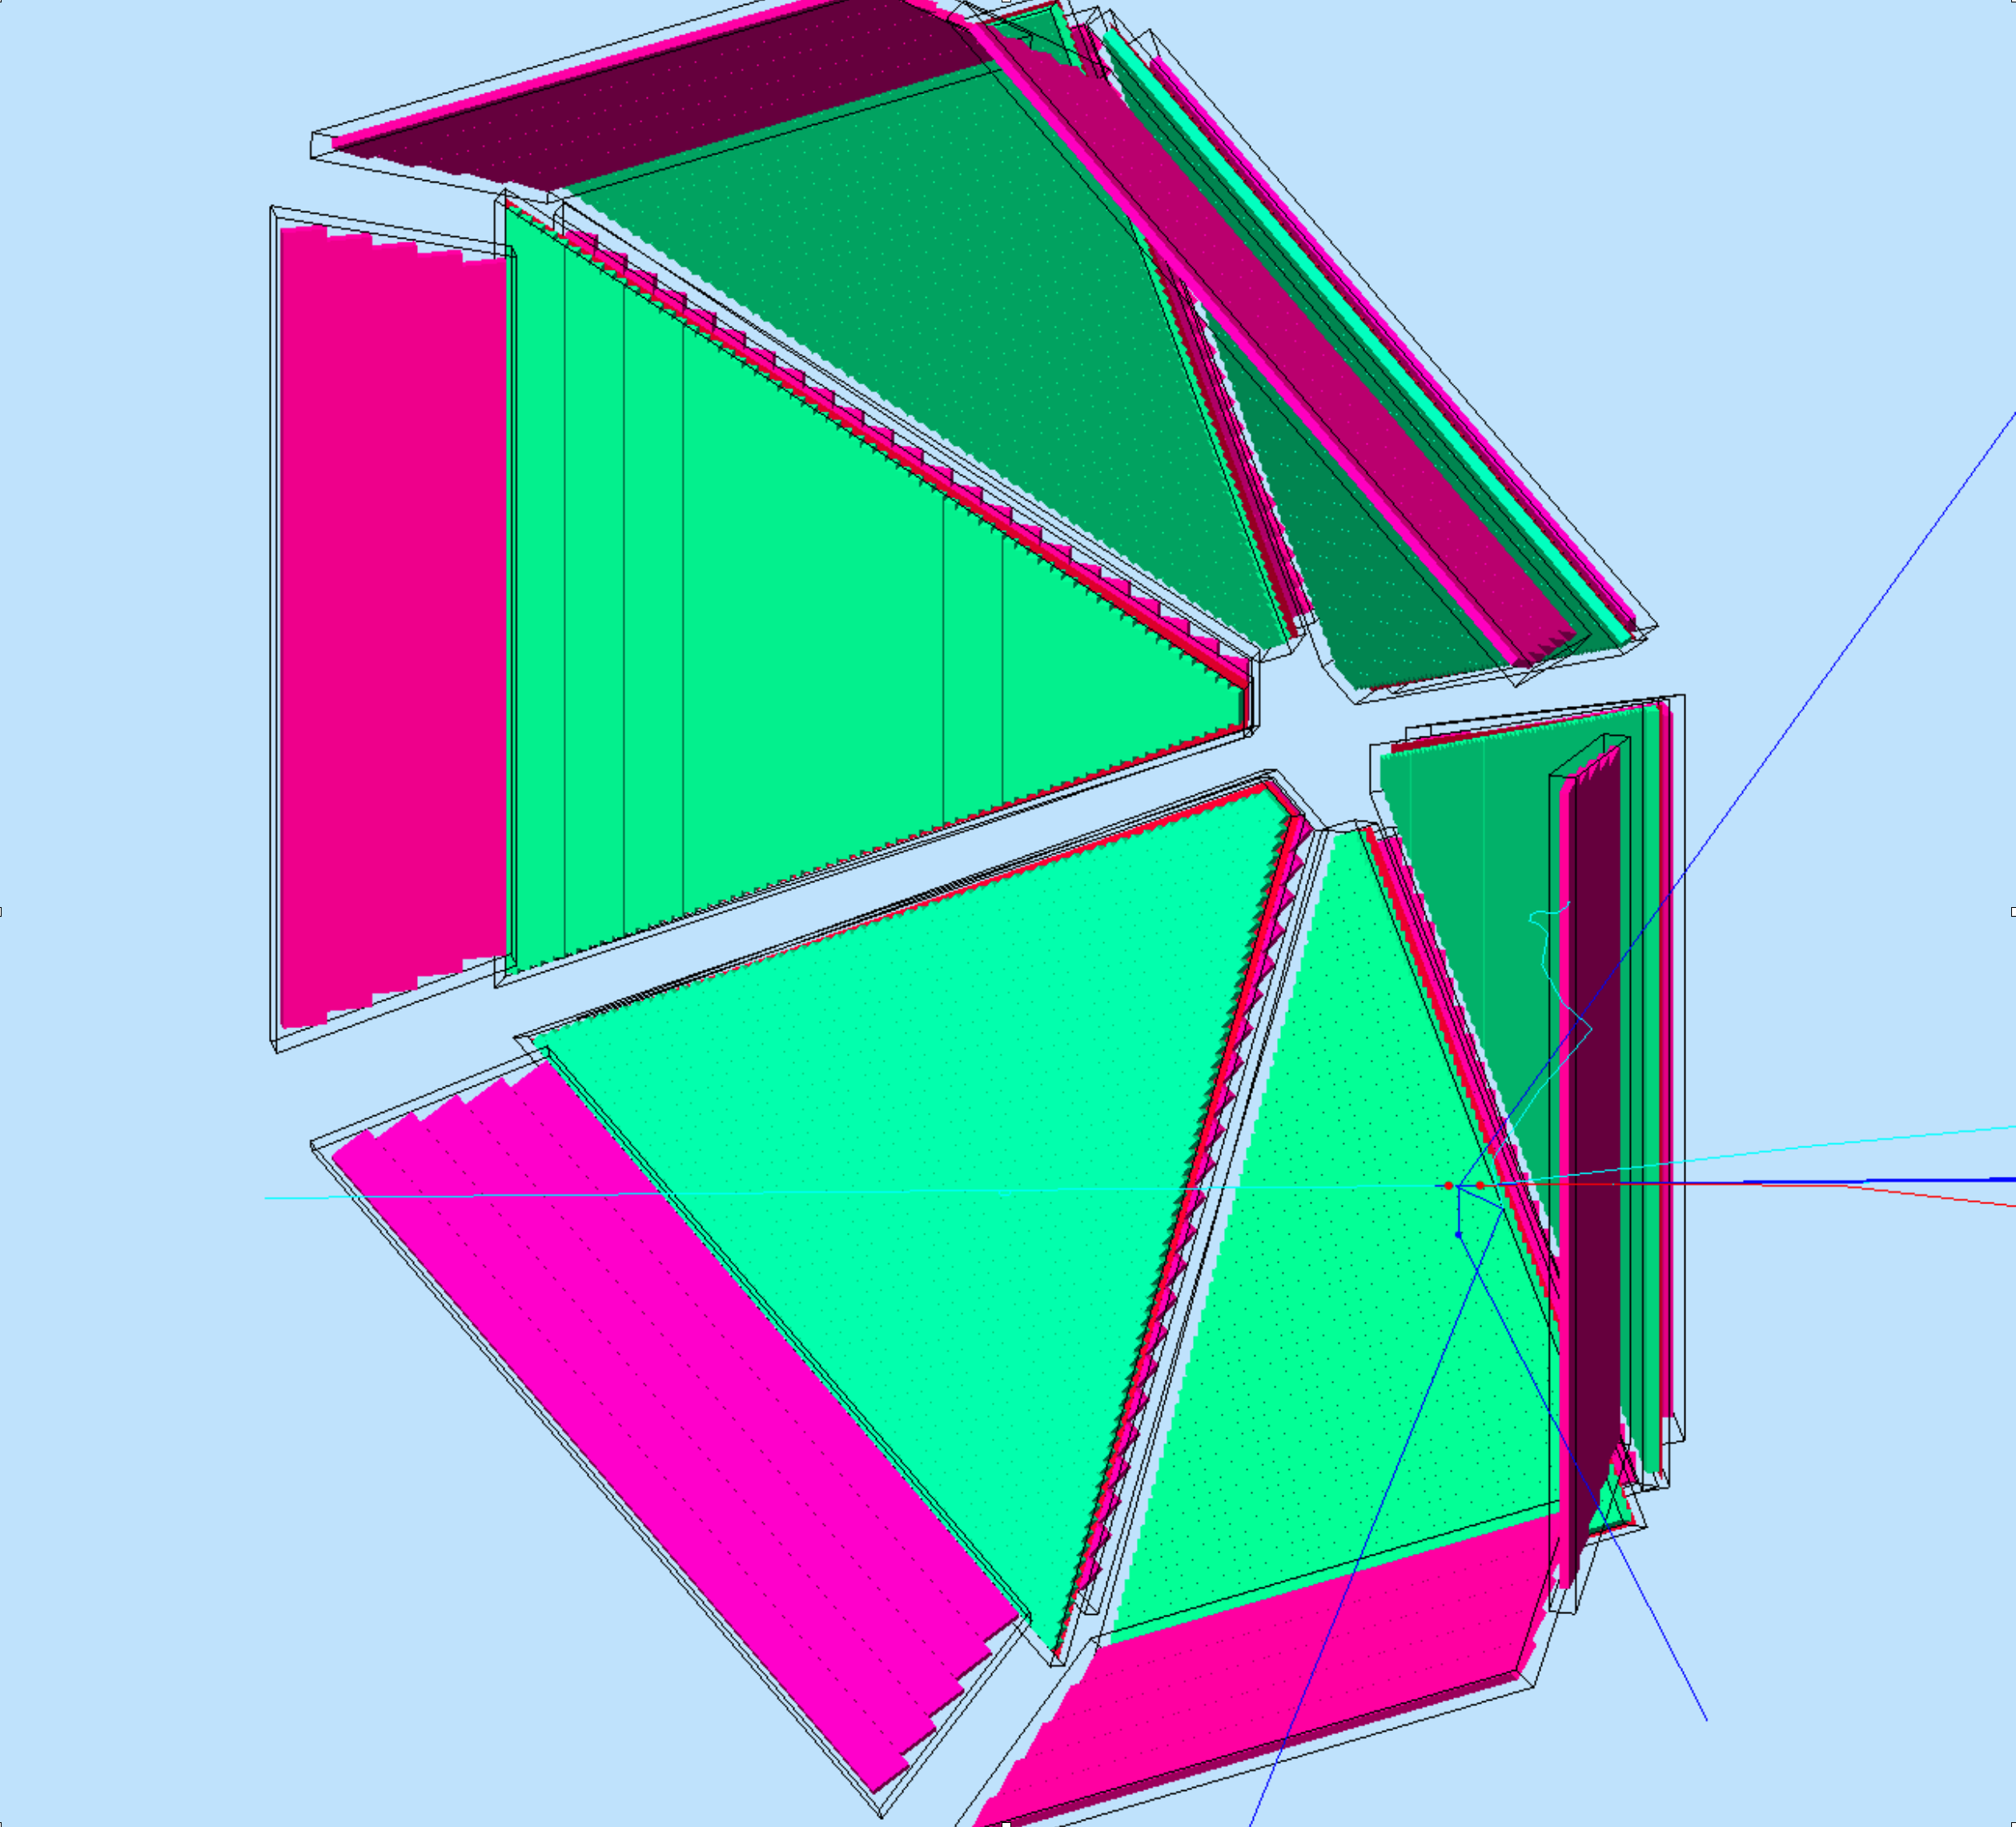
\includegraphics[width=0.99\columnwidth,keepaspectratio]{img/ftofGeometry.png}
	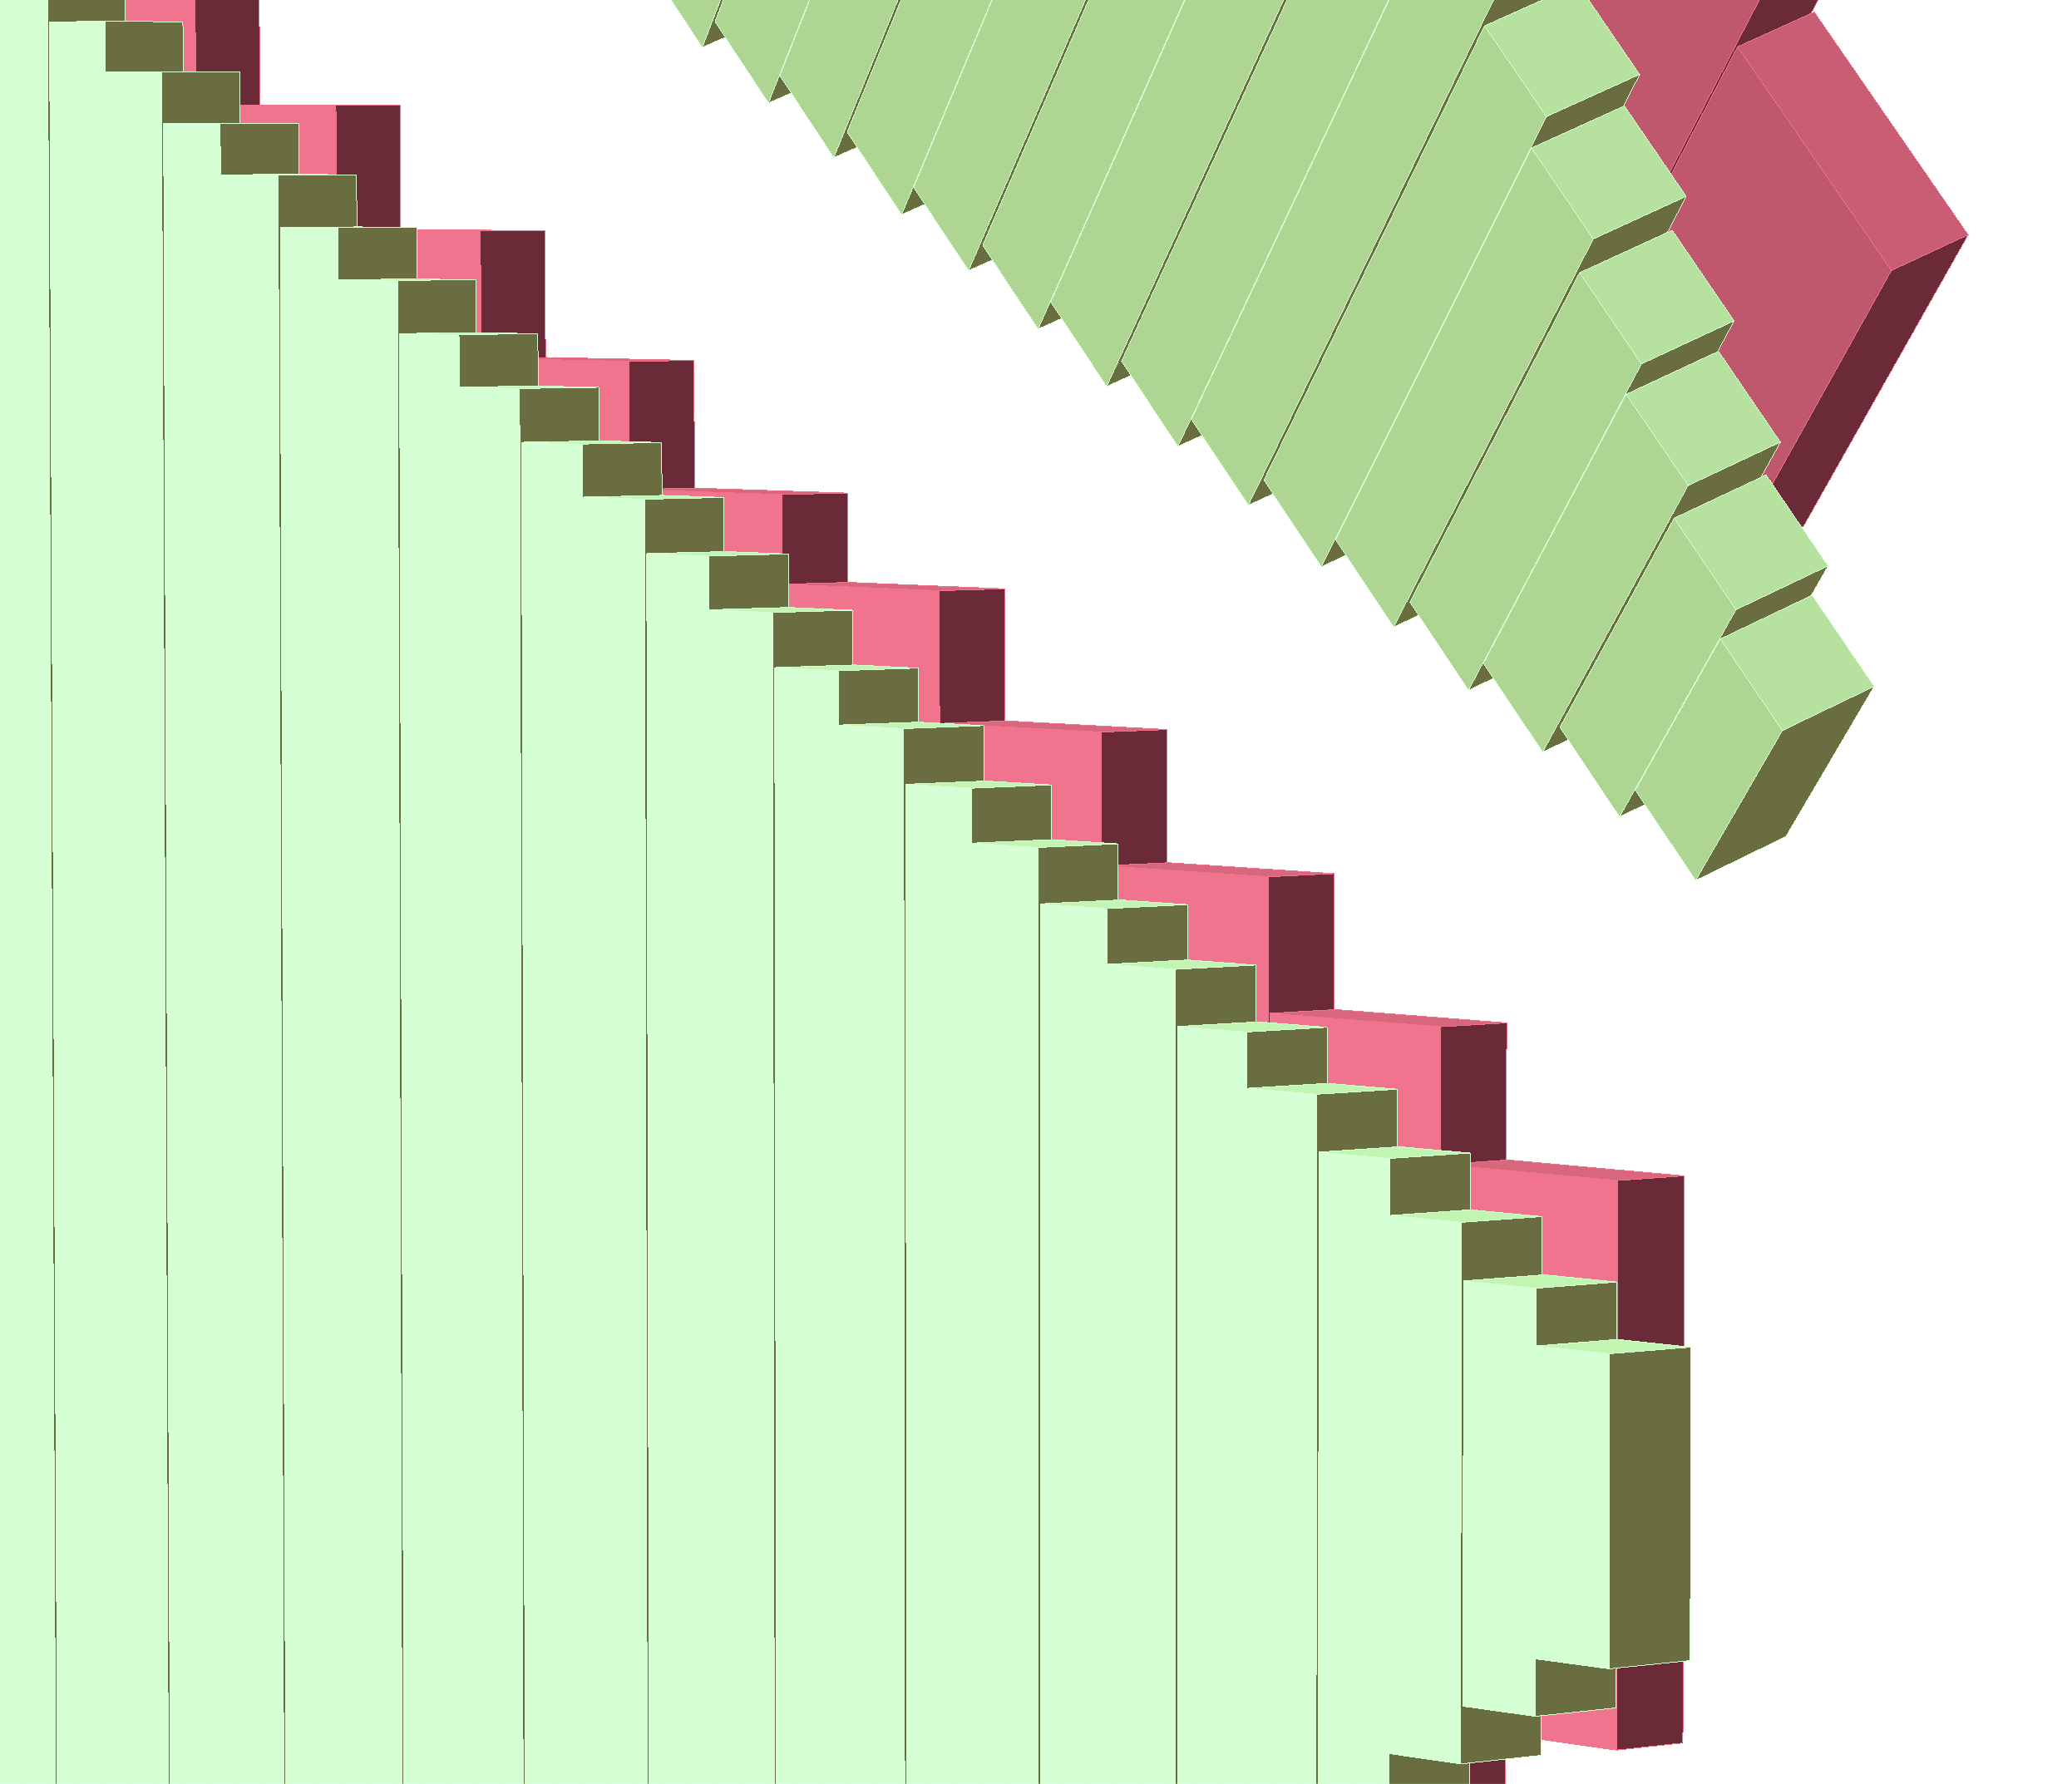
\includegraphics[width=0.99\columnwidth,keepaspectratio]{img/ftofDetail.png}
	\caption{Top: the GEMC implementation of the FTOF geometry. The paddles are G4Boxes, embedded in trapezoid representing the mother volumes of each panel.
            Bottom: a zoom-in of the implementation shows the details of the individual paddles for panel 1B (green) and panel 1A (pink) }
	\label{fig:ftofGeometry}
\end{figure}

\subsubsection{Geometry Location on GitHub}
The Github location of the GEMC perl API script is \url{https://github.com/gemc/detectors/tree/master/clas12/ftof}.
The java geometry service is at \url{https://github.com/JeffersonLab/clas12-offline-software/blob/development/common-tools/clas-jcsg/src/main/java/org/jlab/detector/geant4/v2/FTOFGeant4Factory.java}

\subsection{Process ID}

Each hit in the paddles produces two hits with the identifier variable "side" sets to 0 (for the left side PMT) and 1 (for right side PMT).
The hits are then processed independently through the FTOF hit process routine.

\subsection{Digitization}

\subsubsection{ADC}
The energy deposited is reduced based on the hit position on the paddle using the calibration attenuation length. It is then corrected by a gain factor
to account for the fact that the HV are adjusted so that the geometric ADC mean sqrt(ADCL*ADCR) is independent of counter length and hit position.

The corrected energy is converted to the data derived number of photos $N_{th}$ using the constant 500 $\gamma$ / MeV. A Poissonian is used to
calculate the actual number of photons $N_{actual}$ and the resulting ``smeared`` energy is the converted to ADC using the FADC conversion factor.

An example of the smeared ADC for the right paddles as a function of hit position is shown in \F{ftofAtten}.

\begin{figure}
	\centering
	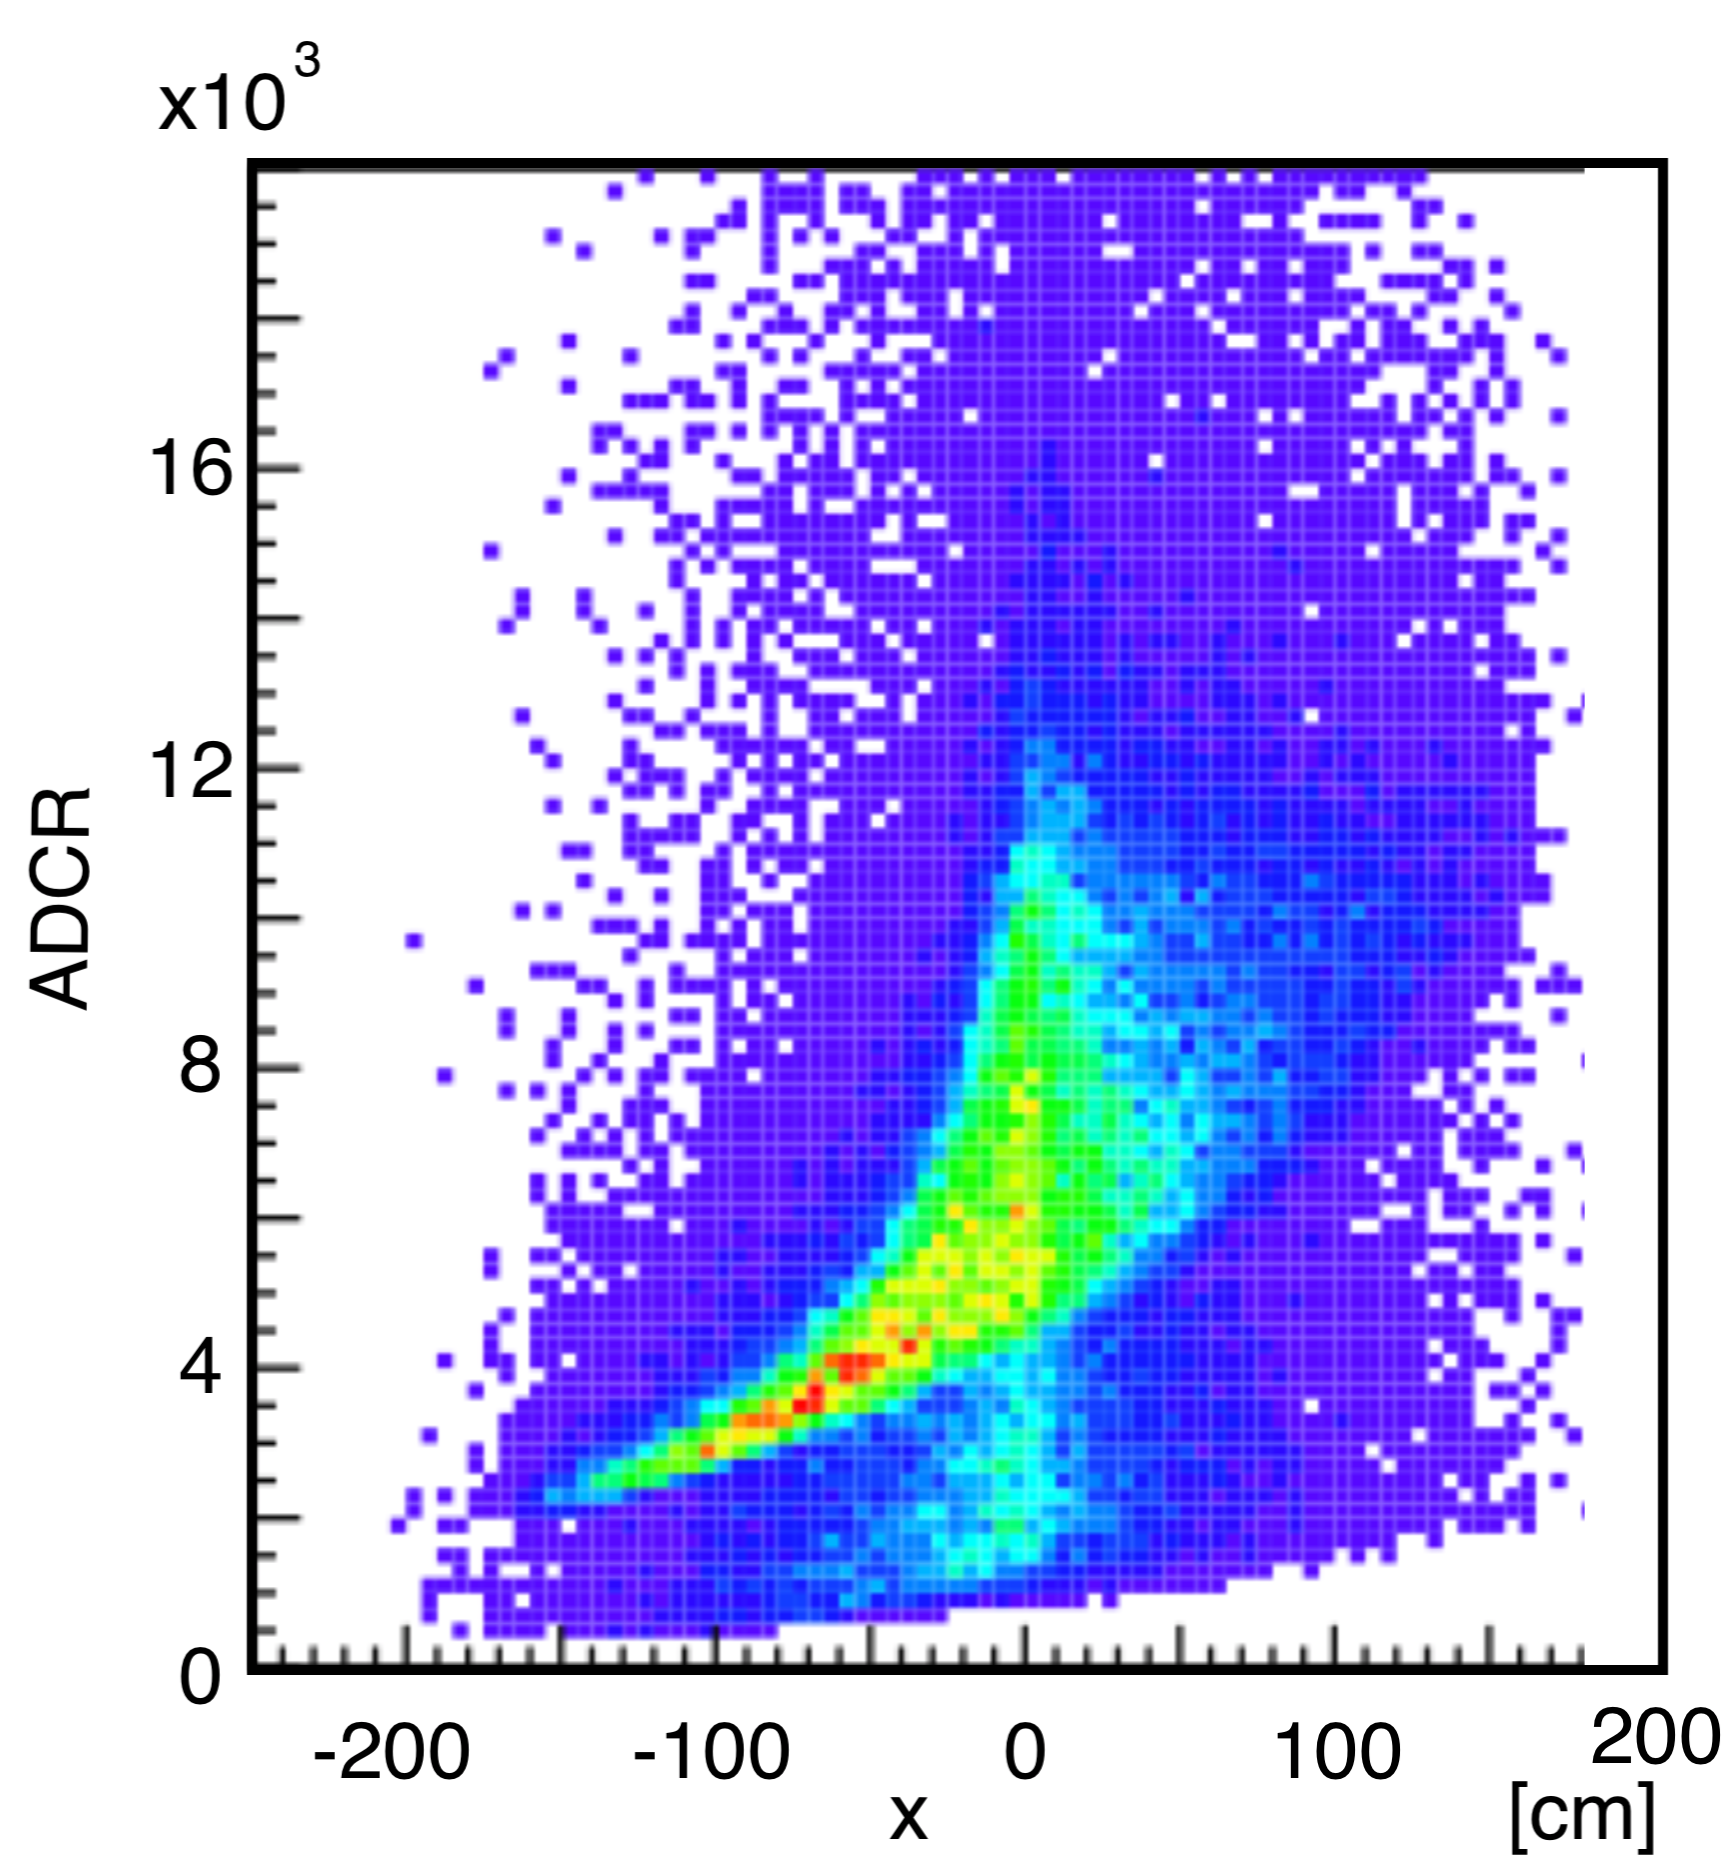
\includegraphics[width=0.99\columnwidth,keepaspectratio]{img/ftofAtten.png}
	\caption{The ADC of the right paddle PMTs as a function of the relative position of the hit in the paddle. The effects of attenuation
				length and smearing using realistic constants from the CCDB database makes the FTOF simulation response very similar to the real data.}
	\label{fig:ftofAtten}
\end{figure}


\subsubsection{TDC}

The absolute hit time is corrected by:

\begin{itemize}
	\item the effective velocity (from CCDB)
	\item the time walk correction, calculated from the smeared energy
	\item a panel to panel timing offset factor (from CCDB)
	\item a left/right time offset factor (from CCDB)
	\item an RF correction (from CCDB)
\end{itemize}

The time is then smeared by a $\sigma$ resolution read from CCDB using a Gaussian function and then digitized using a TDC conversion factor.

\subsubsection{Summary of CCDB Table Used}
\begin{itemize}
	\item /calibration/ftof/attenuation
	\item /calibration/ftof/effective\_velocity
	\item /calibration/ftof/status
	\item /calibration/ftof/gain\_balance
	\item /calibration/ftof/time\_walk
	\item /calibration/ftof/time\_offsets
	\item /calibration/ftof/tdc\_conv
	\item /daq/tt/ftof
\end{itemize}

\subsection{Digitized Bank}
The digitized output bank has $ID=1000$, and the variables are summarized in Table \ref{tab:ftofBank}.

\begin{table}[h]
	\begin{center}
		\begin{tabular}{| c | c | c |}
			\hline \hline
			Variable         & Description  & Tag  \\
			\hline
              sector  &                             sector number  &    1 \\
               layer  &               layer (1: 1A, 2: 1B, 3: 2B)  &    2 \\
              paddle  &                             paddle number  &    3 \\
                side  &                PMT side (0 Left, 1 Right)  &    4 \\
                 ADC  &                                       ADC  &    5 \\
                 TDC  &                                       TDC  &    6 \\
                ADCu  &                             ADC unsmeared  &    7 \\
                TDCu  &                             TDC unsmeared  &    8 \\
                hitn  &                                hit number  &   99 \\
			\hline \hline
		\end{tabular}
	\end{center}
	\caption{The digitized FTOF bank.}\label{tab:ftofBank}
\end{table}


\subsubsection{Time Window}
The time window  of the FTOF is set to 400 ns.

\subsubsection{Process Routine Git Repository Location}
The FTOF hit process routine location in git is \url{https://github.com/gemc/source/blob/master/hitprocess/clas12/ftof_hitprocess.cc}


